\subsection{View}



\subsubsection{de.visaq.view}
\rule{\textwidth}{0.4pt}
\subsubsection {Language}
\begin{minipage}{0.3\textwidth}
    \begin{figure}[H]
        {\centering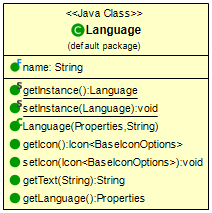
\includegraphics[scale = 0.5
        ]{media/view/view/Language_Class.png}}
    \end{figure}
    \end{minipage} \hfill
    \begin{minipage}{0.6\textwidth}
    Language wird benutzt um die Sprache nach den präferenzen des Benutzers zu setzen. Die Klasse ist nach dem Singelton Entwurfsschema designt.
    \end{minipage}
    \vspace{\baselineskip}
    Attribute: \begin{itemize} [noitemsep]
    \item \emph{public final String name} Name der Sprache
    \end{itemize}
    Methoden: \begin{itemize} [noitemsep]
    \item \emph{public static synchronized Language getInstance()} Gibt die aktuelle Sprach Instanz wieder.
    \item \emph{public static synchronized void setInstance(Language language)} Setzt die aktuelle Sprach Instanz
    \item \emph{public Language(Properties language, String name)} Kosntruktor, welcher die Sprache mit dem gegebenen Namen erstellt und die globele Instanz dementsprechend aktuallisiert.
    \item \emph{public Icon<BaseIconOptions> getIcon()} Gibt das Icon wieder, welches in der Navigationsbar angezeigt wird.
    \item \emph{public void setIcon(Icon<BaseIconOptions> icon)} Setzt das Icon
    \item \emph{public String getText(String key)} Gibt die lokalisierte Version des Property key zurück
    \item \emph{public Properties getLanguage()} Wird benutzt um die Sprach Properties zu erreichen
\end{itemize}

\rule{\textwidth}{0.4pt}
\subsubsection{InformationView}
\begin{minipage}{0.3\textwidth}
    \begin{figure}[H]
        {\centering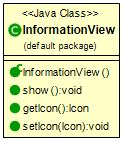
\includegraphics[scale = 0.7
        ]{media/view/view/InformationView_Class.png}}
    \end{figure}
    \end{minipage} \hfill
    \begin{minipage}{0.6\textwidth}
InformationView erstellt die View mit welcher die Benutzer ein hilfestellendes Overlay aktivieren können um so leichter 
die Website zu navigieren.
\end{minipage}
\vspace{\baselineskip}
Methoden: \begin{itemize} [noitemsep]
    \item \emph{public void show()} Zeigt das Hilfeoverlay an
    \item \emph{public Icon getIcon()} Gibt das Icon für die InformationView wieder
    \item \emph{public void setIcon(Icon icon)} Setzt das Icon für die InformationView, bei welchem es sich um ein Icon aus der Bibliothek \gls{Leaflet} handelt.
\end{itemize}

\rule{\textwidth}{0.4pt}
\subsubsection{MapView}
\begin{minipage}{0.5\textwidth}
    \begin{figure}[H]
        {\centering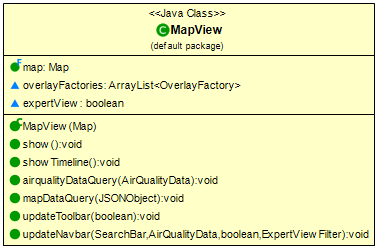
\includegraphics[scale = 0.5
        ]{media/view/view/MapView_Class.png}}
    \end{figure}
    \end{minipage} \hfill
    \begin{minipage}{0.4\textwidth}
MapView erstellt die View für die Karte indem das MapOverlay angezeigt wird. Die Klasse erbt von View und implementiert NavbarObserver und ToolbarObserver.
\end{minipage}
\vspace{\baselineskip}
Attribute: \begin{itemize} [noitemsep]
     \item \emph{public final Map map} Die auf der Website angezeigte Karte
\end{itemize}
Methoden: \begin{itemize} [noitemsep]
    \item \emph{public MapView(Map map)} Ein Kosntruktor welcher die Karte setzt.
    \item \emph{public void show()} Zeigt die Karte und Legende.
    \item \emph{public void timeDataQuery(Instant time)} Eine Datumabfrage, die verwendet wird, wenn der Regeler der Timeline bewegt wird. Die Methode setzt das Datum für die Datenabfrage.
    \item \emph{public void showTimeline()} Zeigt die Historischen Daten und den Regeler für die Timeline
    \item \emph{public void mapDataQueryCoordinates(JSONObject coordinates)} Wird aktiviert, wenn der Benutzer einen Punkt auf der Karte auswählt. Hier werden entweder die Daten des Punkts oder des Sensors angezeigt.
    \item \emph{public void mapDataQuerySensor(Sensor sensor)} Wird aktiviert, wenn der Benutzer einen Sensor auf der Karte auswählt. Hier werden entweder die Daten des Punkts oder des Sensors angezeigt.
    \item \emph{public void update(SearchBar searchBar, AirQualityData currentAirQualityData,
    boolean expertView, ExpertViewFilter expertViewFilter, boolean historicalView)} Updaten falls der Benutzer etwas an den Einstellungen ändert.
    \item \emph{public void airqualityDataQuery(AirQualityData airQualityData)} Eine Abfrage die abfragt was die aktuelle Luftqualitätsdata ist und erstellt dazu die passende Legende. 
\end{itemize} 

\rule{\textwidth}{0.4pt}
\subsubsection{NavbarObserver}
\begin{minipage}{0.4\textwidth}
    \begin{figure}[H]
        {\centering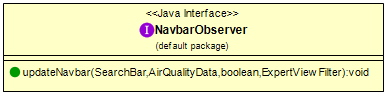
\includegraphics[scale = 0.5
        ]{media/view/view/NavbarObserver_Class.png}}
    \end{figure}
    \end{minipage} \hfill
    \begin{minipage}{0.5\textwidth}
Ein Observer für die Navigationsbar welcher die Instanzen in dieser aktualisiert
\end{minipage}
\vspace{\baselineskip}
Methoden: \begin{itemize} [noitemsep]
    \item \emph{public void update(SearchBar searchbar, AirQualityData currentAirQualityData,
    boolean expertView, ExpertViewFilter expertViewFilter),boolean historicalView} Updaten falls der Benutzer etwas an den Einstellungen ändert.
\end{itemize}

\rule{\textwidth}{0.4pt}
\subsubsection{ObservedNavbarSubject}
\begin{minipage}{0.3\textwidth}
    \begin{figure}[H]
        {\centering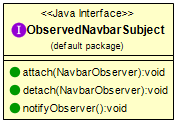
\includegraphics[scale = 0.6
        ]{media/view/view/ObservedNavbarSubject_Class.png}}
    \end{figure}
    \end{minipage} \hfill
    \begin{minipage}{0.6\textwidth}
Ein Interface für das von dem NavbarObserver beobachtete Subjekt, welches den Observer über Änderungen informiert.
\end{minipage}
\vspace{\baselineskip}
Methoden: \begin{itemize} [noitemsep]
    \item \emph{public void attach(NavbarObserver navbarObserver)} Erstellt eine Verbindung zwischen dem Observer und Subjekt her
    \item \emph{public void detach(NavbarObserver navbarObserver)} Entfernt die Verbindung zwischen dem Observer und Subjekt
    \item \emph{public void notifyObserver()} Informiert den Observer über Änderungen
\end{itemize}

\rule{\textwidth}{0.4pt}
\subsubsection{View}
\begin{minipage}{0.3\textwidth}
    \begin{figure}[H]
        {\centering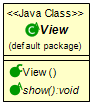
\includegraphics[scale = 0.7
        ]{media/view/view/View_Class.png}}
    \end{figure}
    \end{minipage} \hfill
    \begin{minipage}{0.6\textwidth}
Eine abstrakte Klasse welche regelt wie die Website für den Benutzer dargestellt wird. Das beinhaltet die unterschiedlichen Sprachen und die ColorTheme. Außerdem implementiert die Klasse NavbarObserver.
\end{minipage}
\vspace{\baselineskip}
Methoden: \begin{itemize} [noitemsep]
    \item \emph{public void show()} Zeigt die Website an
\end{itemize}

\rule{\textwidth}{0.4pt}
\subsubsection{VisAQ}
\begin{minipage}{0.3\textwidth}
    \begin{figure}[H]
        {\centering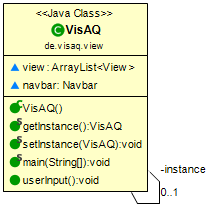
\includegraphics[scale = 0.5
        ]{media/view/view/VisAQ_Class.png}}
    \end{figure}
    \end{minipage} \hfill
    \begin{minipage}{0.6\textwidth}
Die Main Klasse der Anwendung. Hier ist der Einstieg in die Anwendung, welcher die Eingaben des Benutzers weitergibt und die View öffnet. Dies erfolgt über das Springframework.
\end{minipage}
\vspace{\baselineskip}
Methoden: \begin{itemize} [noitemsep]
    \item \emph{public static void main(String[] args)} Die main Methode der Anwendung.
\end{itemize} 

\rule{\textwidth}{0.4pt}
\subsection{de.view.elements}

\rule{\textwidth}{0.4pt}
\subsubsection{CookieNotice}
\begin{minipage}{0.3\textwidth}
    \begin{figure}[H]
        {\centering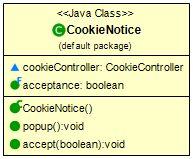
\includegraphics[scale = 0.5
        ]{media/view/CookieNotice_Class.png}}
    \end{figure}
    \end{minipage} \hfill
    \begin{minipage}{0.6\textwidth}
Popup, welches den Benutzer darüber informiert, dass VisAQ Cookies nach dem EU Recht verwendet
\end{minipage}
\vspace{\baselineskip}
Attribute: \begin{itemize} [noitemsep]
     \item \emph{CookieController cookieController} Ein neuer CookieController
    \item \emph{public final boolean acceptance} Ein boolean Attribut, welches verwendet wird um zu entscheiden ob der Benutzer die Cookies akzeptiert oder nicht
\end{itemize}
Methoden: \begin{itemize} [noitemsep]
    \item \emph{public CookieNotice()} Konstruktor für die CookieNotice
    \item \emph{public popup()} Das Pupup Fenster welches beim laden der Website die CookieNotice anzeigt und dem Benutzer erlaubt die Cookies zu akzeptieren
    \item \emph{public void accept(boolean acceptance)} Gibt dem CookieController weiter, dass der Benutzer die Cookies akzeptiert oder nicht
\end{itemize}


\rule{\textwidth}{0.4pt}
\subsection{de.view.elements.airquality}

\rule{\textwidth}{0.4pt}
\subsubsection{AirQualityData}
\begin{minipage}{0.3\textwidth}
    \begin{figure}[H]
        {\centering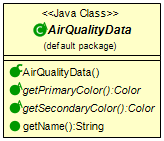
\includegraphics[scale = 0.6
        ]{media/view/airquality/AirQualityData_Class.png}}
    \end{figure}
    \end{minipage} \hfill
    \begin{minipage}{0.6\textwidth}
Objekt welches dafür verwendet wird die unterschiedlichen Farbschemata für die Legenden darzustellen.
\end{minipage}
\vspace{\baselineskip}
Attribute: \begin{itemize} [noitemsep]
     \item \emph{public static final String NAME} The name of the AirQualityData
\end{itemize}
Methoden: \begin{itemize} [noitemsep]
    \item \emph{public abstract Color getPrimaryColor()} The primary color that is used in order to create the gradient in the legend
    \item \emph{public abstract Color getSecondaryColor()} The secondary color that is used in order to create the gradient in that legend
\end{itemize}

\rule{\textwidth}{0.4pt}
\subsubsection{ParticulateMatter}
\begin{minipage}{0.3\textwidth}
    \begin{figure}[H]
        {\centering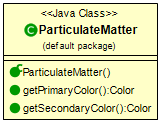
\includegraphics[scale = 0.6
        ]{media/view/airquality/ParticulateMatter_Class.png}}
    \end{figure}
    \end{minipage} \hfill
    \begin{minipage}{0.6\textwidth}
ParticulateMatter erstellt die Einstellungen für die Messungen gemessen von den Sensoren. Die Klasse erbt von AirQualityData.
\end{minipage}
\vspace{\baselineskip}
Methoden: \begin{itemize} [noitemsep]
	\item \emph{public abstract Color getPrimaryColor()} Die Primärfarbe welche dafür verwendet wird um den Farbverlauf in der Legende zu erstellen.
	\item \emph{public abstract Color getSecondaryColor()} Die Sekundärfarbe welche dafür verwendet wird um den Farbverlauf in der Legende zu erstellen.
\end{itemize}

\rule{\textwidth}{0.4pt}
\subsubsection{Temperature}
\begin{minipage}{0.3\textwidth}
    \begin{figure}[H]
        {\centering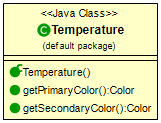
\includegraphics[scale = 0.6
        ]{media/view/airquality/Temperature_Class.png}}
    \end{figure}
    \end{minipage} \hfill
    \begin{minipage}{0.6\textwidth}
Temperature erstellt die Einstellungen für die Messungen gemessen von den Sensoren. Die Klasse erbt von AirQualityData.
\end{minipage}
\vspace{\baselineskip}
Methoden: \begin{itemize} [noitemsep]
	\item \emph{public abstract Color getPrimaryColor()} Die Primärfarbe welche dafür verwendet wird um den Farbverlauf in der Legende zu erstellen.
	\item \emph{public abstract Color getSecondaryColor()} Die Sekundärfarbe welche dafür verwendet wird um den Farbverlauf in der Legende zu erstellen.
\end{itemize}

\rule{\textwidth}{0.4pt}
\subsubsection{Humidity}
\begin{minipage}{0.3\textwidth}
    \begin{figure}[H]
        {\centering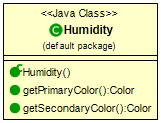
\includegraphics[scale = 0.6
        ]{media/view/airquality/Humidity_Class.png}}
    \end{figure}
    \end{minipage} \hfill
    \begin{minipage}{0.6\textwidth}
Humidity erstellt die Einstellungen für die Messungen gemessen von den Sensoren. Die Klasse erbt von AirQualityData.
\end{minipage}
\vspace{\baselineskip}
Methoden: \begin{itemize} [noitemsep]
	\item \emph{public abstract Color getPrimaryColor()} Die Primärfarbe welche dafür verwendet wird um den Farbverlauf in der Legende zu erstellen.
	\item \emph{public abstract Color getSecondaryColor()} Die Sekundärfarbe welche dafür verwendet wird um den Farbverlauf in der Legende zu erstellen.
\end{itemize}

\rule{\textwidth}{0.4pt}
\subsubsection{AirPressure}
\begin{minipage}{0.3\textwidth}
    \begin{figure}[H]
        {\centering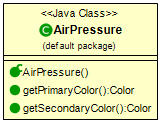
\includegraphics[scale = 0.6
        ]{media/view/airquality/AirPressure_Class.png}}
    \end{figure}
    \end{minipage} \hfill
    \begin{minipage}{0.6\textwidth}
AirPressure erstellt die Einstellungen für die Messungen gemessen von den Sensoren. Die Klasse erbt von AirQualityData.
\end{minipage}
\vspace{\baselineskip}
Methoden: \begin{itemize} [noitemsep]
    \item \emph{public abstract Color getPrimaryColor()} Die Primärfarbe welche dafür verwendet wird um den Farbverlauf in der Legende zu erstellen.
    \item \emph{public abstract Color getSecondaryColor()} Die Sekundärfarbe welche dafür verwendet wird um den Farbverlauf in der Legende zu erstellen.
\end{itemize}


\rule{\textwidth}{0.4pt}
\subsection{de.view.elements.diagram}

\rule{\textwidth}{0.4pt}
\subsubsection{Diagram}
\begin{minipage}{0.3\textwidth}
    \begin{figure}[H]
        {\centering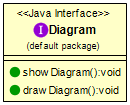
\includegraphics[scale = 0.7
        ]{media/view/diagram/Diagram_Class.png}}
    \end{figure}
    \end{minipage} \hfill
    \begin{minipage}{0.6\textwidth}
Das Diagram Interface erstellt das Diagramm für die SensorOverview. Es handelt sich hierbei um ein Interface
\end{minipage}
\vspace{\baselineskip}
Methoden: \begin{itemize} [noitemsep]
    \item \emph{public void showDiagram()} Zeigt Diagram an
    \item \emph{public void drawDiagram()} Zeichnet das Diagramm
\end{itemize}

\rule{\textwidth}{0.4pt}
\subsubsection{BarDiagram}
\begin{minipage}{0.3\textwidth}
    \begin{figure}[H]
        {\centering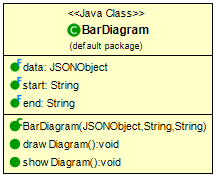
\includegraphics[scale = 0.5
        ]{media/view/diagram/BarDiagram_Class.png}}
    \end{figure}
    \end{minipage} \hfill
    \begin{minipage}{0.6\textwidth}
BarDiagram erstellt ein Balkendiagramm für Diagram und implementiert dieses.
\end{minipage}
\vspace{\baselineskip}
Attribute: \begin{itemize} [noitemsep]
    \item \emph{public final JSONObject data} Ein JSON Objekt, welches die Daten an das Diagram weitergibt.
    \item \emph{public final String start} Der Start der angezeigten historischen Werte im Diagram
    \item \emph{public final String end} Das Ende der angezeigten historischen Werte im Diagram
\end{itemize}
Methoden: \begin{itemize} [noitemsep]
    \item \emph{public BarDiagram(JSONObject data, String start, String end)} Der Konstruktor für das Balkendiagramm, welcher mit dem JSONObject und dem Start und dem Ende initialisiert wird
    \item \emph{public void showDiagram()} Zeigt Diagram an
    \item \emph{public void drawDiagram()} Zeichnet das Diagramm
\end{itemize}

\rule{\textwidth}{0.4pt}
\subsubsection{LineDiagram}
\begin{minipage}{0.3\textwidth}
    \begin{figure}[H]
        {\centering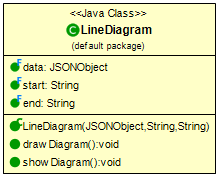
\includegraphics[scale = 0.5
        ]{media/view/diagram/LineDiagram_Class.png}}
    \end{figure}
    \end{minipage} \hfill
    \begin{minipage}{0.6\textwidth}
BarDiagram erstellt ein Liniendiagramm für Diagram und implementiert dieses.
\end{minipage}
\vspace{\baselineskip}
Attribute: \begin{itemize} [noitemsep]
    \item \emph{public final JSONObject data} Ein JSON Objekt, welches die Daten an das Diagram weitergibt.
    \item \emph{public final String start} Der Start der angezeigten historischen Werte im Diagram
    \item \emph{public final String end} Das Ende der angezeigten historischen Werte im Diagram
\end{itemize}
Methoden: \begin{itemize} [noitemsep]
    \item \emph{public BarDiagram(JSONObject data, String start, String end)} Der Konstruktor für das Balkendiagramm, welcher mit dem JSONObject und dem Start und dem Ende initialisiert wird
    \item \emph{public void showDiagram()} Zeigt Diagram an
    \item \emph{public void drawDiagram()} Zeichnet das Diagramm
\end{itemize}

\rule{\textwidth}{0.4pt}
\subsection{de.view.elements.map}

\rule{\textwidth}{0.4pt}
\subsubsection{Legend}
\begin{minipage}{0.3\textwidth}
    \begin{figure}[H]
        {\centering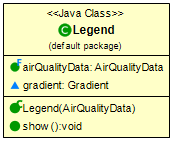
\includegraphics[scale = 0.5
        ]{media/view/map/Legend_Class.png}}
    \end{figure}
    \end{minipage} \hfill
    \begin{minipage}{0.6\textwidth}
Die Legende zeigt die Farbskala für die auf der Karte angezeigten Interpolationswerte. Die Legende ändert ihre Farbwerte je nach ausgewählter Luftqualitätsdata
\end{minipage}
\vspace{\baselineskip}
Attribute: \begin{itemize} [noitemsep]
     \item \emph{public final AirQualityData airQualityData} Die von dem Benutzer ausgewählte Luftqualitätsdata
\end{itemize}
Methoden: \begin{itemize} [noitemsep]
    \item \emph{public Legend(AirQualityData airQualityData)} Konstruktor für die Legende für die ausgewählte Luftqualitätsdata
    \item \emph{public void show()} Zeigt die aktuelle Legende an
\end{itemize}

\rule{\textwidth}{0.4pt}
\subsubsection{SensorOverview}
\begin{minipage}{0.3\textwidth}
    \begin{figure}[H]
        {\centering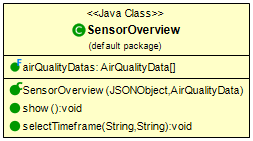
\includegraphics[scale = 0.5
        ]{media/view/map/SensorOverview_Class.png}}
    \end{figure}
    \end{minipage} \hfill
    \begin{minipage}{0.6\textwidth}
SensorOverview (auch Sidebar genannt) wird benutzt um die Interpolierten Point Data auf der Karte sowie die Daten eines speziellen Sensors anzuzeigen. Es zeigt ein Diagramm mit historischen Werten an, welche von dem Benutzer individuell gewählt werden können. Außerdem werden die Gefahren von den spezifischen Arten von Luftverschmutzung angezeigt, sowie die von dem Sensor gemessenen Werte.
\end{minipage}
\vspace{\baselineskip}
Attribute: \begin{itemize} [noitemsep]
    \item \emph{public final AirQualityData[] airQualityDatas} Ein Array mit den vier AirQualityDaten
\end{itemize}
Methoden: \begin{itemize} [noitemsep]
    \item \emph{public SensorOverview(JSONObject coordinates, AirQualityData currentAirQualityData)} Konstruktor für die Sidebar mit den Koordinaten und der zurzeit ausgewählten Luftqualitätsdata
    \item \emph{public void show()} Zeigt die Sidebar
    \item \emph{public void selectTimeframe(String start, String end)} Die von dem Benutzer ausgewählte Zeit
    \item \emph{public Diagram getDiagram()} Gibt das Diagramm wieder.
    \item \emph{public void setDiagram(Diagram diagram)} Setzt das Diagramm
\end{itemize}

\rule{\textwidth}{0.4pt}
\subsection{de.view.elements.navbar}

\rule{\textwidth}{0.4pt}
\subsubsection{ExpertViewFilter}
\begin{minipage}{0.3\textwidth}
    \begin{figure}[H]
        {\centering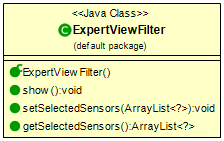
\includegraphics[scale = 0.55
        ]{media/view/navbar/ExpertviewFilter_Class.png}}
    \end{figure}
    \end{minipage} \hfill
    \begin{minipage}{0.6\textwidth}
ExpertViewFilter ist eine Erweiterung für erfahrene Benutzer, welche bei Aktivierung in der Navigationsbar auswählen können welche Sensortypen sie angezeigt haben wollen.
\end{minipage}
\vspace{\baselineskip}
Methoden: \begin{itemize} [noitemsep]
    \item \emph{public void show()} Zeigt die Möglichkeit an, an welcher man den Experten Modus an beziehungsweise ausmachen kann.
    \item \emph{public void setSelectedSensors(ArrayList<?> selectedSensorTypes)} Setzt die von dem Benutzer ausgewählten Sensortypen
    \item \emph{public ArrayList<?> getSelectedSensors()} Gibt die ausgewählten SensorTypen weiter.
\end{itemize}

\rule{\textwidth}{0.4pt}
\subsubsection{Navbar}
\begin{minipage}{0.5\textwidth}
    \begin{figure}[H]
        {\centering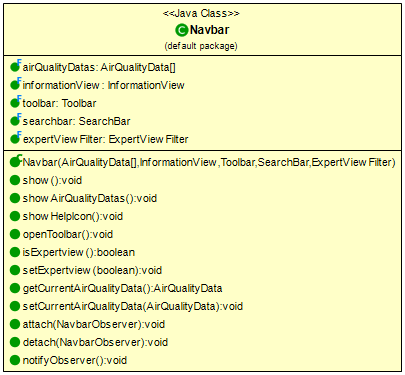
\includegraphics[scale = 0.45
        ]{media/view/navbar/Navbar_Class.png}}
    \end{figure}
    \end{minipage} \hfill
    \begin{minipage}{0.5\textwidth}
Die Navbar zeigt die Navigationsbar und erlaubt es dem Benutzer auf die Hilfe, Suchleiste, Sprache, Toolbar und die Luftqualitätsfilter zuzugreifen
\end{minipage}
\vspace{\baselineskip}
Attribute:\begin{itemize} [noitemsep]
    \item \emph{public final AirQualityData[] airQualityDatas} Array welches die 4 Luftqualitätsdata beinhaltet
    \item \emph{public final InformationView informationView} Die InformationView die angezeigt wird
    \item \emph{public final Toolbar toolbar} Die Toolbar die angezeigt wird
    \item \emph{public final SearchBar searchbar} Die Suchleiste die angezeigt wird
    \item \emph{public final ExpertViewFilter expertViewFilter} In dem ExpertViewFilter kann der Benutzer unterschiedliche Sensor Typen auswählen
\end{itemize}
Methoden: \begin{itemize} [noitemsep]
    \item \emph{public Navbar(AirQualityData[] airQualityDatas, InformationView informationView, Toolbar toolbar, SearchBar searchbar, ExpertViewFilter expertViewFilter)} Konstruktor für eine neue Navigationsbar
    \item \emph{public void show()} Zeigt die Suchleiste
    \item \emph{public void showAirQualityDatas()} Shows the available Air Quality Data overlays.
    \item \emph{public void showHelpIcon()} Zeigt das Hilfe-Icon
    \item \emph{public void openToolbar()} Zeigt die Toolbar
    \item \emph{public boolean isExpertview()} Informiert ob der Experten Modus ausgewählt ist oder nicht.
    \item \emph{public void setExpertview(boolean expertview)} Aktiviert oder deaktiviert den Experten Modus
    \item \emph{public AirQualityData getCurrentAirQualityData()} Gibt die aktuelle Luftqualitätsdata zurück
    \item \emph{public void setCurrentAirQualityData(AirQualityData currentAirQualityData)} Setzt die aktuelle Luftqualitätsdata
    \item \emph{public void attach(NavbarObserver navbarObserver)} Fügt einen Navigationsbar Observer hinzu
    \item \emph{public void detach(NavbarObserver navbarObserver)} Entfernt einen Navigationsbar Observer.
    \item \emph{public void notifyObserver()} Gibt dem Observer weiter was in der Navigationbar passiert.
\end{itemize}

\rule{\textwidth}{0.4pt}
\subsubsection{SearchBar}
\begin{minipage}{0.3\textwidth}
    \begin{figure}[H]
        {\centering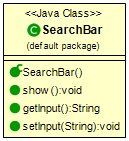
\includegraphics[scale = 0.65]{media/view/navbar/Searchbar_Class.png}}
    \end{figure}
    \end{minipage} \hfill
    \begin{minipage}{0.6\textwidth}
Suchleiste die der Benutzer benutzen kann um nach bestimmten Städten oder Postleitzahlen zu suchen
\end{minipage}
\vspace{\baselineskip}
Methoden: \begin{itemize} [noitemsep]
    \item \emph{public Seachbar()} Konstruktor für die Suchleiste.
    \item \emph{public void show()}  Zeigt die Suchleiste in der Navbar an
    \item \emph{public String getInput()} Gibt den Benutzer input weiter und erlaubt die weitere Benutzung dieser.
    \item \emph{public void setInput(String input)} Setzt den Suchleisten input
\end{itemize}

\rule{\textwidth}{0.4pt}
\subsection{de.view.elements.toolbar}

\rule{\textwidth}{0.4pt}
\subsubsection{Timeline}
\begin{minipage}{0.3\textwidth}
    \begin{figure}[H]
        {\centering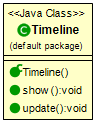
\includegraphics[scale = 0.7
        ]{media/view/toolbar/Timeline_Class.png}}
    \end{figure}
    \end{minipage} \hfill
    \begin{minipage}{0.6\textwidth}
Die Timeline ist ein Regulator welcher aufgerufen werden kann und die historischen Daten direkt auf der Karte darstellt. Es implementiert außerdem ToolbarElement um die dazugehörige show Methode zu verwenden.
\end{minipage}
\vspace{\baselineskip}
Methoden: \begin{itemize} [noitemsep]
    \item \emph{public void show()} Zeigt die Timeline an, wenn diese von dem Benutzer ausgewählt wurde.
    \item \emph{public void update()} Aktualisiert das Overlay je nach ausgewählten historischen Daten.
\end{itemize}

\rule{\textwidth}{0.4pt}
\subsubsection{Toolbar}
\begin{minipage}{0.3\textwidth}
    \begin{figure}[H]
        {\centering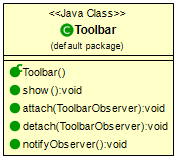
\includegraphics[scale = 0.5
        ]{media/view/toolbar/Toolbar_Class.png}}
    \end{figure}
    \end{minipage} \hfill
    \begin{minipage}{0.6\textwidth}
Zeigt dem Benutzer die einzelnen Links und Beschreibungen zu den einzelnen Funktionen
\end{minipage}
\vspace{\baselineskip}
Methoden: \begin{itemize} [noitemsep]
    \item \emph{public Toolbar()} Konstruktor für die Toolbar
    \item \emph{public void show()} Zeigt die Toolbar
    \item \emph{public void attach(ToolbarObserver toolbarObserver)}
    \item \emph{public void detach(ToolbarObserver toolbarObserver)}
    \item \emph{public void notifyObserver()}
\end{itemize}

\rule{\textwidth}{0.4pt}
\subsubsection{ToolbarElement}
\begin{minipage}{0.3\textwidth}
    \begin{figure}[H]
        {\centering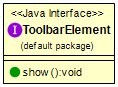
\includegraphics[scale = 0.7
        ]{media/view/toolbar/ToolbarElement.png}}
    \end{figure}
    \end{minipage} \hfill
    \begin{minipage}{0.6\textwidth}
Interface für alle Elemente welche in der Toolbar gezeigt werden können.
\end{minipage}
\vspace{\baselineskip}
Methoden: \begin{itemize} [noitemsep]
    \item \emph{public void show()} Zeigt die einzelnen Elemente auf der Schnittstelle
\end{itemize}

\rule{\textwidth}{0.4pt}
\subsection{de.view.overlay.factory}

\rule{\textwidth}{0.4pt}
\subsubsection{OverlayFactory}
\begin{minipage}{0.3\textwidth}
    \begin{figure}[H]
        {\centering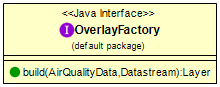
\includegraphics[scale = 0.6
        ]{media/view/factory/OverlayFactory_Class.png}}
    \end{figure}
    \end{minipage} \hfill
    \begin{minipage}{0.6\textwidth}
Kapselt die Kontrolle über die Overlay factories
\end{minipage}
\vspace{\baselineskip}
Methoden: \begin{itemize} [noitemsep]
    \item \emph{public Layer build(AirQualityData airquality,  Datastream datastream)}  Baut einen Overlay mithilfe von der aktuellen Luftqualitätsdata
\end{itemize}

\rule{\textwidth}{0.4pt}
\subsubsection{InterpolationOverlayFactory}
\begin{minipage}{0.3\textwidth}
    \begin{figure}[H]
        {\centering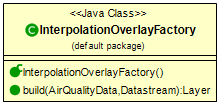
\includegraphics[scale = 0.5
        ]{media/view/factory/InterpolationOverlayFactory_Class.png}}
    \end{figure}
    \end{minipage} \hfill
    \begin{minipage}{0.6\textwidth}
Erstellt ein Map Overlay welches die unterschiedlichen Interpolationswerte anzeigt die von unterschiedlichen Sensoren gemessen werden.
\end{minipage}
\vspace{\baselineskip}
Methoden: \begin{itemize} [noitemsep]
    \item \emph{public Layer build(AirQualityData airquality,  Datastream datastream)} Baut einen Overlay mithilfe von der aktuellen Luftqualitätsdata
\end{itemize}
    \rule{\textwidth}{0.4pt}
\subsubsection{SensorOverlayFactory}
\begin{minipage}{0.3\textwidth}
    \begin{figure}[H]
        {\centering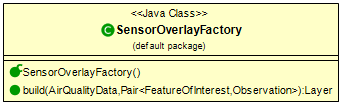
\includegraphics[scale = 0.5
        ]{media/view/factory/SensorOverlayFactory_Class.png}}
    \end{figure}
    \end{minipage} \hfill
    \begin{minipage}{0.6\textwidth}
        Erstellt ein Map Overlay welches die unterschiedlichen Sensordata anzeigt die von unterschiedlichen Sensoren gemessen werden.
\end{minipage}
\vspace{\baselineskip}
 Methoden: \begin{itemize} [noitemsep]
    \item \emph{public Layer build(AirQualityData airquality,  Datastream datastream)} Baut einen Overlay mithilfe von der aktuellen Luftqualitätsdata
\end{itemize}

\rule{\textwidth}{0.4pt}
\subsubsection{OverlayBuilder}
\begin{minipage}{0.5\textwidth}
    \begin{figure}[H]
        {\centering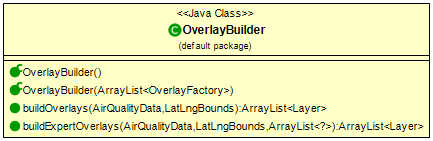
\includegraphics[scale = 0.5
        ]{media/view/factory/OverlayBuilder_Class.png}}
    \end{figure}
    \end{minipage} \hfill
    \begin{minipage}{0.4\textwidth}
Schnittstelle füt die Overlay factory. Hier werden die Overlays mithilfe von speziellen factories für die Karten gebaut
\end{minipage}
\vspace{\baselineskip}
Methoden: \begin{itemize} [noitemsep]
    \item \emph{public OverlayBuilder()} Standard Builder, welcher Overlay Factory und Interpolation Overlay Factory verwendet.
    \item \emph{public OverlayBuilder(ArrayList<OverlayFactory> factories)} Builder für das bauen von Overlays mithilfe von factories.
    \item \emph{public ArrayList<Layer> buildOverlays(AirQualityData airquality, LatLngBounds latLngBounds)} Erstellt eine ArrayList mit den unterschiedlichen Layern anhand der ausgewählten Luftqualitätsdata und den Bounds.
\end{itemize}


\rule{\textwidth}{0.4pt}
\subsection{de.view.elements.theme}

\rule{\textwidth}{0.4pt}
\subsubsection{ColorTheme}
\begin{minipage}{0.3\textwidth}
    \begin{figure}[H]
        {\centering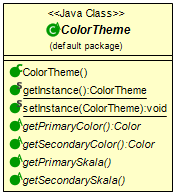
\includegraphics[scale = 0.5
        ]{media/view/theme/ColorTheme_Class.png}}
    \end{figure}
    \end{minipage} \hfill
    \begin{minipage}{0.6\textwidth}
ColorTheme ist eine Funktion mit welcher der Benutzer die Farben wechseln kann in welchen die Schnittstelle dargestellt wird. Die Klasse wurde nach einem Singelton Entwurfsmuster designt
\end{minipage}
\vspace{\baselineskip}
Methoden: \begin{itemize} [noitemsep]
    \item \emph{public ColorTheme()} Erstellt eine ColorTheme Instanz und aktualisiert diese.
    \item \emph{public static synchronized ColorTheme getInstance()} Gibt einen Wert von dem Typ ColorTheme zurück
    \item \emph{public static synchronized void setInstance(ColorTheme colorTheme)} Setzt die aktuelle ColorTheme Instanz
    \item \emph{public abstract Color getPrimaryColor()} Gibt einen Wert von dem Typ Color zurück
    \item \emph{public abstract Color getSecondaryColor()} Gibt einen Wert von dem Typ Color zurück
    \item \emph{public abstract Gradient getPrimarySkala()} Gibt einen Wert von dem Typ Gradient zurück
    \item \emph{public abstract Gradient getSecondarySkala()}  Gibt einen Wert von dem Typ Gradient zurück
\end{itemize}

\rule{\textwidth}{0.4pt}
\subsubsection{DarkTheme}
\begin{minipage}{0.3\textwidth}
    \begin{figure}[H]
        {\centering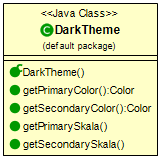
\includegraphics[scale = 0.5
        ]{media/view/theme/DarkTheme_Class.png}}
    \end{figure}
    \end{minipage} \hfill
    \begin{minipage}{0.6\textwidth}
       Ein dunkleres Farbschema für die Visualisierung der Website.
    \end{minipage}
    \vspace{\baselineskip}
Methoden: \begin{itemize} [noitemsep]
    \item \emph{public ColorTheme()} Erstellt eine ColorTheme Instanz und aktualisiert diese.
    \item \emph{public static synchronized ColorTheme getInstance()} Gibt einen Wert von dem Typ ColorTheme zurück
    \item \emph{public static synchronized void setInstance(ColorTheme colorTheme)} Setzt die aktuelle ColorTheme Instanz
    \item \emph{public abstract Color getPrimaryColor()} Gibt einen Wert von dem Typ Color zurück
    \item \emph{public abstract Color getSecondaryColor()} Gibt einen Wert von dem Typ Color zurück
    \item \emph{public abstract Gradient getPrimarySkala()} Gibt einen Wert von dem Typ Gradient zurück
    \item \emph{public abstract Gradient getSecondarySkala()}  Gibt einen Wert von dem Typ Gradient zurück
\end{itemize}

\rule{\textwidth}{0.4pt}
\subsubsection{LightTheme}
\begin{minipage}{0.3\textwidth}
    \begin{figure}[H]
        {\centering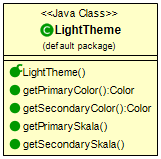
\includegraphics[scale = 0.5
        ]{media/view/theme/LightTheme_Class.png}}
    \end{figure}
    \end{minipage} \hfill
    \begin{minipage}{0.6\textwidth}
        Ein helleres Farbschema für die Visualisierung der Website. Dieses wird bei einem Erstbesuch als Standardschema geladen.
    \end{minipage}
    \vspace{\baselineskip}
Methoden: \begin{itemize} [noitemsep]
    \item \emph{public ColorTheme()} Erstellt eine ColorTheme Instanz und aktualisiert diese.
    \item \emph{public static synchronized ColorTheme getInstance()} Gibt einen Wert von dem Typ ColorTheme zurück
    \item \emph{public static synchronized void setInstance(ColorTheme colorTheme)} Setzt die aktuelle ColorTheme Instanz
    \item \emph{public abstract Color getPrimaryColor()} Gibt einen Wert von dem Typ Color zurück
    \item \emph{public abstract Color getSecondaryColor()} Gibt einen Wert von dem Typ Color zurück
    \item \emph{public abstract Gradient getPrimarySkala()} Gibt einen Wert von dem Typ Gradient zurück
    \item \emph{public abstract Gradient getSecondarySkala()}  Gibt einen Wert von dem Typ Gradient zurück
\end{itemize}

\rule{\textwidth}{0.4pt}
\subsubsection{ColorBlindTheme}
\begin{minipage}{0.3\textwidth}
\begin{figure}[H]
    {\centering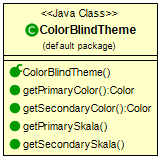
\includegraphics[scale = 0.5
    ]{media/view/theme/ColorBlindTheme_Class.png}}
\end{figure}
\end{minipage} \hfill
\begin{minipage}{0.6\textwidth}
    Ein Farbblindenschema für die Visualisierung der Website. In diesem Fall speziell für eine Rot-Grün Sehschwäche.
\end{minipage}
\vspace{\baselineskip}
Methoden: \begin{itemize} [noitemsep]
    \item \emph{public ColorTheme()} Erstellt eine ColorTheme Instanz und aktualisiert diese.
    \item \emph{public static synchronized ColorTheme getInstance()} Gibt einen Wert von dem Typ ColorTheme zurück
    \item \emph{public static synchronized void setInstance(ColorTheme colorTheme)} Setzt die aktuelle ColorTheme Instanz
    \item \emph{public abstract Color getPrimaryColor()} Gibt einen Wert von dem Typ Color zurück
    \item \emph{public abstract Color getSecondaryColor()} Gibt einen Wert von dem Typ Color zurück
    \item \emph{public abstract Gradient getPrimarySkala()} Gibt einen Wert von dem Typ Gradient zurück
    \item \emph{public abstract Gradient getSecondarySkala()}  Gibt einen Wert von dem Typ Gradient zurück
\end{itemize}

\rule{\textwidth}{0.4pt}
\subsubsection{Gradient} 
\begin{minipage}{0.3\textwidth}
    \begin{figure}[H]
    {\centering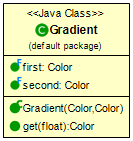
\includegraphics[scale = 0.6
    ]{media/view/theme/Gradient_Class.png}}
    \end{figure}
    \end{minipage} \hfill
    \begin{minipage}{0.6\textwidth}
    Beschreibt einen Farbverlauf zwischen zwei Punkten. Und kann auf die spezifischen Farbwerte im Farbverlauf zugreifen.
    \end{minipage}
    \vspace{\baselineskip}
Attribute: \begin{itemize} [noitemsep]
     \item \emph{public final Color first} Die Primärfarbe für das erstellen des Farbverlaufs.
    \item \emph{public final Color second} Die Sekundärfarbe für das erstellen des Farbverlaufs.
\end{itemize}
Methoden: \begin{itemize} [noitemsep]
    \item \emph{public Gradient(Color first, Color second)} Konstruktor, welcher mithilfe der Primärfarbe und Sekundärfarbe den Farbverlauf erstellt.
    \item \emph{public Color get(float at)} Gibt eine Farbe zurück, welche zwischen * 100 Prozent der Primärfarbe und Sekundärfarbe liegt und mithilfe von linearer Interpolation.
\end{itemize}

\rule{\textwidth}{0.4pt}